\chapter{Implementation}
\label{chap:implementation}

This chapter will focus on the implementation details of the project. It will cover the pipeline framework, the pipelines themselves, and the mosaicing process.

Having decided to focus on Fourier domain approaches, the two obvious candidates to implement are both \citeauthor{Reddy1996}'s and \citeauthor{Hurtos2015}'s pipelines. There are some modifications, improvements, and optimizations that have been made to the basic implementations and will be presented in the following sections.

Additionally, a few restrictions/assumptions are set:

\begin{itemize}
    \item All the frames should have the same range and number of beams. 
    \item The drone is assumed to never change its diving depth.
\end{itemize}

All of the code for the whole implementation is available at: https://github.com/jp-pino/sonar-registration.

\section{A Small Comment on Pipelines and Code}

\begin{figure}[H] 
  \centering
  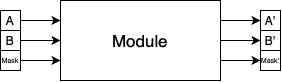
\includegraphics[width=.75\textwidth]{figures/Module.png}
  \caption{A Module, the main building block of a pipeline.}
\end{figure}

Since the pipelines are composed of mostly independent modules that operate on two input images and in some cases, their mask, a flexible framework has been designed to model this behaviour. A \textit{pipeline} contains a sequence of modules that by default are fed the output of the preceding one. This behavior can be modified to suit the pipeline's needs by specifying the module's id whose output will be chosen as input. Pipelines themselves can be used as modules to organize the code better. A small example of the syntax used for the registration section of the Fourier-Mellin Pipeline is shown below:

\begin{lstlisting}[
    caption={Example of pipeline definition.},
    label=lst:pipeline-definition,
    language=Python]
registration_id, registration = Pipeline('registration')
start_id, _ = registration.add_module(IdentityModule())
registration.add_module(FourierModule())
registration.add_module(LogPolarModule(order=1))
registration.add_module(PhaseCorrelationModule(10, 'rotation'))
registration.add_module(IdentityModule(), input_stage=start_id)
registration.add_module(WarpModule(), apply_to=('b', 'm'))
registration.add_module(PhaseCorrelationModule(10, 'translation'))
\end{lstlisting}

The \lstinline{add_module} method on the pipeline allows us to specify a module, the input stage, and to which of the inputs apply the functionality. The rerouteable inputs work by caching the output of each module in the pipeline itself. If rerouting is specified, the pipeline will use these cached values instead of using the output of the previous module. In addition, the pipeline itself, on initialization, can take arguments to aid in debugging by printing the output of the pipeline at that stage. Hopefully, this will make it easier to iterate on or modify the code by swapping out modules or extending pipelines. All this functionality, however, comes with the additional cost of memory to hold the cached values of the pipeline during the cycle. A fully optimized, monolithic pipeline would be more efficient and might be the right step when working towards implementing this in the \acrshort{rov}, however, this approach offers the flexibility needed during this experimentation phase.

In most cases, the modules perform the same operations on the inputs, in which case it would be advantageous to perform these tasks in parallel. To simplify the implementation of parallelization, the modules use \texttt{Ray} from Anyscale, Inc. Processing only on the CPU is not the most efficient, but by parallelizing the pipeline where possible some speedup can be gained.

Parallelization using \texttt{Ray} is done using \texttt{Tasks}. These turn static methods into asynchronously executable functions, ideally helping us to halve the time it takes to execute a module. In essence, any static function is a candidate for this. Note the \lstinline{@ray.remote} in the following example of a module using \texttt{Ray}:

\begin{lstlisting}[
    caption={Example of pipeline parallelization.},
    label=lst:pipeline-parallelization,
    language=Python]
class BandpassModule(PipelineModule):
    def __init__(self, low_cutoff, high_cutoff):
        super().__init__()
        self.low_cutoff = low_cutoff
        self.high_cutoff = high_cutoff

    @staticmethod
    @ray.remote
    def bandpass(data, low_cutoff, high_cutoff):
        if data is None:
            return None
        return difference_of_gaussians(data, low_cutoff, high_cutoff)

    def run(self, a, b, mask, tform, error):
        a = self.bandpass.remote(a, self.low_cutoff, self.high_cutoff)
        b = self.bandpass.remote(b, self.low_cutoff, self.high_cutoff)
        return ray.get(a), ray.get(b), mask, tform, error
\end{lstlisting}

As can be seen in this example, the module inherits from \texttt{PipelineModule}. In fact, all Modules and Pipelines inherit from this class. It provides a common interface for accessing the \texttt{run} method, and keep track of module-identifying information.

The \lstinline{run} method takes in, and returns, five parameters. Two frames (a and b), the mask, a transform that describes the rotation and translation, and an error array containing three elements; the registration error for the x and y axes, and rotation. This is what allows the modules to be chained. The Pipeline class acts as a manager, piping the correct outputs to the correct inputs, and caching all results.  


\section{\citeauthor{Reddy1996}'s Fourier-Mellin Pipeline (adapted)}
\label{sec:fmpipeline}
\begin{figure}[H] 
  \centering
  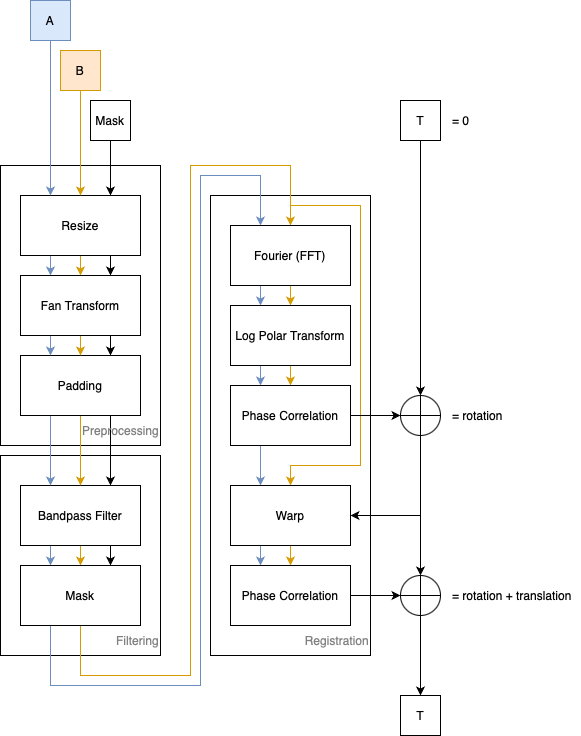
\includegraphics[width=.9\textwidth]{figures/fourier_mellin_pipeline.png}
  \caption{Block diagram of the Fourier-Mellin registration pipeline (adapted).}
  \label{fig:fmpipeline}
\end{figure}

The Fourier-Mellin Pipeline has been adapted to suit sonar images in a total of 10 independent modules. The main adaptation is the addition of the first block of modules (Resizing, Fan Transformation, and Padding) which allows the Fourier-Mellin Pipeline to work on sonar images. Note that most of them are fed their inputs sequentially, except for the Warp Module which applies the detected rotation to the masked image so that the translation could be identified. Here, the flexibility of the pipeline framework implementation shines. The next sections will go into more detail about how each module is implemented. 

\begin{lstlisting}[
    caption={Fourier-Mellin Pipeline Implementation.},
    label=lst:fm-pipeline-code,
    language=Python]
pipeline = Pipeline(output=args.out, 
                    intermediate_output=args.intermediate_output, 
                    verbose=args.verbose)
pipeline.add_module(IdentityModule())
conditioning_id, conditioning = pipeline.add_module(Pipeline('conditioning'))
conditioning.add_module(ResizeModule(args.resize))
conditioning.add_module(FanModule(bearings, output=args.out))
conditioning.add_module(PaddingModule(0.25))

pipeline.add_module(MetricsModule(output=args.out))

filtering_id, filtering = pipeline.add_module(Pipeline('filtering'))
filtering.add_module(BandpassModule(args.bandpass_low, args.bandpass_high))
filtering.add_module(MaskModule(padding=60, sigma=15))

registration_id, registration = pipeline.add_module(Pipeline('registration'))
start_id, _ = registration.add_module(IdentityModule())
registration.add_module(FourierModule())
registration.add_module(LogPolarModule(order=1))
registration.add_module(PhaseCorrelationModule(10, 'rotation'))
registration.add_module(IdentityModule(), input_stage=start_id)
registration.add_module(WarpModule(), apply_to=('b', 'm'))
registration.add_module(PhaseCorrelationModule(10, 'translation'))

pipeline.add_module(UpdateTformModule(range_resolution=range_resolution))
pipeline.add_module(IdentityModule(), ('a', 'b'), input_stage=conditioning_id)
pipeline.add_module(WarpModule(combine=True), 'b')
pipeline.add_module(OdometerModule(output=args.out, 
                                   range_resolution=range_resolution))
\end{lstlisting}

Although the specifics of each module will be described in the following sections, the process in this pipeline can be summarized in the following steps:
\begin{enumerate}
    \item Convert the raw sonar data into processed fan-shaped frames. Here small optimizations like resizing and padding take place.
    \item Features in this sonar frame are enhanced using a Bandpass Filter, namely the \acrfull{dog}. This will make it less likely for the pipeline to fixate on the noise. 
    \item Some degree of masking is applied to the fan-shaped frame to reduce the spectral leakage from the edges of the fan.
    \item Rotation is estimated using a combination of \acrshort{fft}, Log-Polar Transform, and Phase Correlation. This rotation estimation is fully decoupled from the translation, making it robust in registering distant frames.
    \item The estimated rotation is applied to the incoming frame so that pure translation can be estimated using Phase Correlation once more.
\end{enumerate}

\section{\citeauthor{Hurtos2015}'s Raw Polar Pipeline}
\begin{figure}[H] 
  \centering
  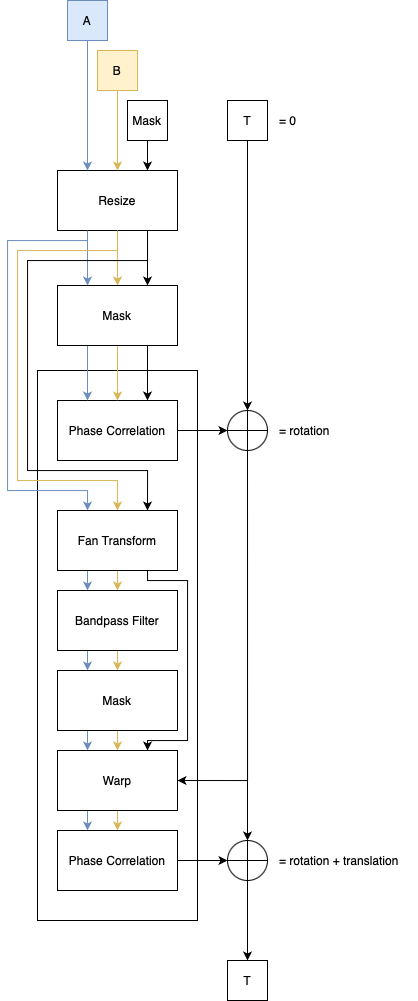
\includegraphics[width=.7\textwidth]{figures/pc_pipeline.png}
  \caption{Block diagram of the Raw Polar Pipeline (adapted).}
  \label{fig:pcpipeline}
\end{figure}

With 9 modules the Raw Polar Pipeline isn't much shorter on first inspection. On a closer look, however, it is evident that some of the heavyweight modules from the Fourier-Mellin pipeline are missing: Fourier Transform and the Log-Polar transform. As mentioned before, performing Phase Correlation over the raw polar image although faster, might not perform so well on distant frames. This is because the rotation isn't decoupled from the translation in the raw sonar frame. 

Given the frequency of sonar frames coming from the \acrshort{bsosonar} (see \autoref{tab:sonar_specs}) and the max speed of the drone (see \autoref{tab:drone_specs}, we can assume that translations will be very small. At \(10Hz\) there is \(0.1s\) between frames. At the maximum speed of the drone\(1.5m/s\) the maximum movement between frames would be \(0.15m\). This is a small value indeed, but will most probably be much lower given that to improve accuracy the drone will be driven in slow settings. 

\begin{lstlisting}[
    caption={Raw Polar Pipeline Implementation.},
    label=lst:pc-pipeline-code,
    language=Python]
pipeline = Pipeline(output=args.out, 
                    intermediate_output=args.intermediate_output, 
                    verbose=args.verbose)
registration_id, registration = pipeline.add_module(Pipeline('registration'))
registration.add_module(ResizeModule(args.resize))
resize_id, _ = registration.add_module(IdentityModule())
registration.add_module(MaskModule(padding=60, sigma=15))
registration.add_module(PhaseCorrelationModule(20, 'rotation', log_polar=False))
registration.add_module(FanModule(bearings, output=args.out), input_stage=resize_id)
padding_id, _ = registration.add_module(PaddingModule(0.25))
registration.add_module(BandpassModule(args.bandpass_low, args.bandpass_high))
registration.add_module(MaskModule(padding=60, sigma=15))
registration.add_module(WarpModule(), apply_to=('b', 'm'))
registration.add_module(PhaseCorrelationModule(10, 'translation'))
pipeline.add_module(UpdateTformModule())
pipeline.add_module(IdentityModule(), ('a', 'b'), input_stage=pipeline.name)
pipeline.add_module(OdometerModule(output=args.out, 
                                   range_resolution=range_resolution))
pipeline.add_module(IdentityModule(), input_stage=padding_id)
pipeline.add_module(WarpModule(combine=True), 'b')
\end{lstlisting}

Similar to the previous pipeline, the process can be summarized in a couple steps:
\begin{itemize}
    \item The raw frames are used to estimate rotation. This involves applying Phase Correlation over the masked image. This mask is not fan-shapped, but actually square.
    \item Once the rotation has been estimated, the raw data from the frame is converted into the processed fan. The rotation is applied to ready it for the next step.
    \item Using Phase Correlation once more, translation is calculated. 
\end{itemize}

\section{Pre-Processing Pipelines' Modules}

Many modules are used in both pipelines and are worth mentioning here.
\begin{itemize}
    \item Resizing: mainly down-sampling, is essential for speeding up the processing pipeline as it reduces the computations needed down the line. Often the starting point of the pipeline. Taking as input a resizing ratio \(R\) it calculates the expected size of the resized image and re-scales it appropriately. Down-sampling with an anti-aliasing filter also also reduces noise, another positive side-effect of this module.
    \item Padding: necessary for keeping the sonar image in frame once the rotation is applied. A black border is added to the image to keep the relevant data in frame.
    \item Filtering: it is recommended to apply some degree of band-pass filtering focusing in particular on high frequency noise.
    \item Masking: the images should be windowed to have smooth borders to avoid spectral leakage from the image borders. This module applies some gaussian filtering to the current mask and applies it to the input images. This makes the image have a smoother transition from the border to the data.
\end{itemize}


\subsection{Resizing (down-sampling)}

\begin{figure}[H]
    \centering
    \begin{subfigure}[b]{.45\textwidth}
        \centering
        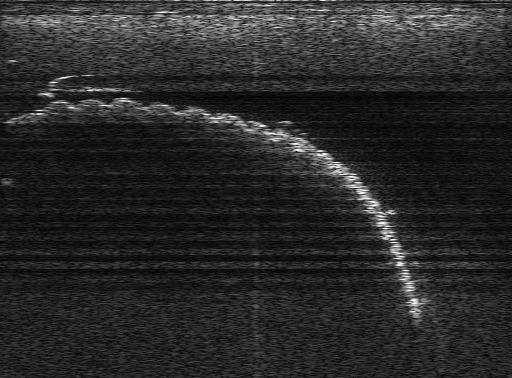
\includegraphics[width=\textwidth]{figures/pipeline/Original.png}
        \caption{Raw data obtained from the sonar.}
    \end{subfigure}
    \hfill
    \begin{subfigure}[b]{.45\textwidth}
        \centering
        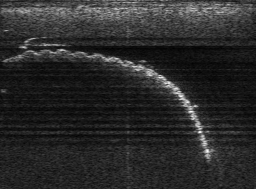
\includegraphics[width=\textwidth]{figures/pipeline/Resized.png}
        \caption{Resized frame.}
    \end{subfigure}
    \caption{Down-sampled image.}
    \label{fig:resizing}
\end{figure}

Resizing the images is necessary to make the pipelines in consideration less computationally expensive. This is a "low hanging fruit" optimization that yields visible results. This module takes images of size \((w, h)\) and re-scales them to \((w^*, h^*)\), given a resizing ratio \(R\) where:

\[w^* = w\sqrt{R}\]
\[h^* = h\sqrt{R}\]

In code this is achieved using the \texttt{skimage.transform.resize} package using:

\begin{lstlisting}[
    caption={Resizing code.},
    label=lst:pipeline-resizing,
    language=Python]
ratio = np.sqrt(R)
img = resize(img.copy(), 
             (int(img.shape[0] * ratio), int(img.shape[1] * ratio)), 
             anti_aliasing=True)
\end{lstlisting}

The \lstinline{anti_aliasing=True} is necessary to avoid the introduction of aliasing artifacts through down-sampling. Down-sampling an image has the secondary function of acting as a kind of averaging filter which will also work towards reducing the noise in the image. 

Later on, in the results section, the speedup (\autoref{sec:speedup}) resulting from down-sampling of the image will be evaluated. It is also important to mention that since operations are done independently on each input image, this is a perfect candidate for parallelization over its inputs with \texttt{Ray}.

\subsection{Padding}

\begin{figure}[H]
    \centering
    \begin{subfigure}[b]{.45\textwidth}
        \centering
        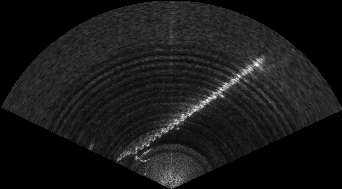
\includegraphics[width=\textwidth]{figures/pipeline/Fan.png}
        \caption{Input fan frame.}
    \end{subfigure}
    \hfill
    \begin{subfigure}[b]{.45\textwidth}
        \centering
        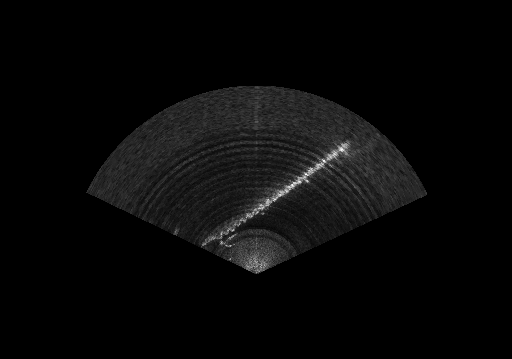
\includegraphics[width=\textwidth]{figures/pipeline/Padding.png}
        \caption{Padded fan frame.}
    \end{subfigure}
    \caption{Padded image.}
\end{figure}

Especially necessary for images that have undergone their Fan Transformation and will be rotated. Any rotation applied to the image might make some of its data go beyond the edges. Adding some padding ensures that all the sonar data remains inside the image. The module takes in a padding ratio \(r\) and pads the image with a black border with a width of \(r * max(widht, height)\). By default, the padding ratio is chosen to be \texttt{0.25}. Smaller values could be chosen, but this may affect registration of distant frames. Choosing this parameter depends on two things: how distant the frames are (big rotations and translations) and the computational impact of more pixels downstream in the pipeline.

In code this is implemented using numpy as:
\begin{lstlisting}[
    caption={Padding code.},
    label=lst:pipeline-padding,
    language=Python]
pad_size = int(np.max(img.shape) * self.padding_ratio)
np.pad(data, pad_size, mode='constant', constant_values=0)
\end{lstlisting}

Again, since there are no dependecies between the images, this is a perfect candidate for parallelization using \texttt{Ray}.

\section{Filtering}

\begin{figure}[H]
    \centering
    \begin{subfigure}[b]{.45\textwidth}
        \centering
        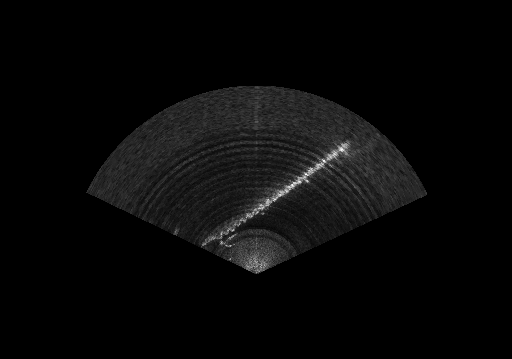
\includegraphics[width=\textwidth]{figures/pipeline/Padding.png}
        \caption{Input padded fan frame.}
    \end{subfigure}
    \hfill
    \begin{subfigure}[b]{.45\textwidth}
        \centering
        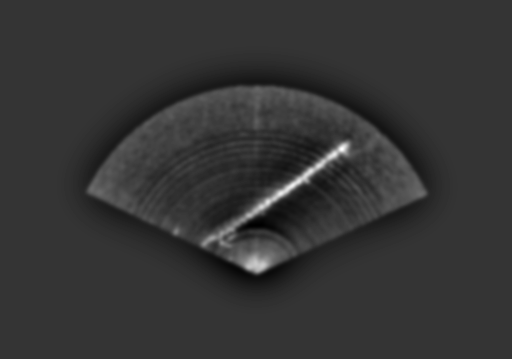
\includegraphics[width=\textwidth]{figures/pipeline/Bandpass.png}
        \caption{Band-passed padded fan frame.}
    \end{subfigure}
    \caption{Band-passed image.}
\end{figure}

If required by the pipeline, a band-pass filter has been implemented using \acrfull{dog}. This is a spatial-domain band-pass filter that also works as a feature enhancement algorithm. The filter generates two blurred versions of the original using Gaussian blur, where one of the images is more blurred than the other. The output results from subtracting the more blurry image from the less blurry one. It can enhance edges and other details present in the image while attenuating the noise, making it perfect for image registration.

The \acrshort{dog} takes two parameters \(\sigma_{low}\) and \(\sigma_{high}\). Choosing these values was done qualitatively to include some blurring and maximize contrast with features in the image.

\begin{figure}[H]
    \centering
    \begin{subfigure}[b]{.32\textwidth}
        \centering
        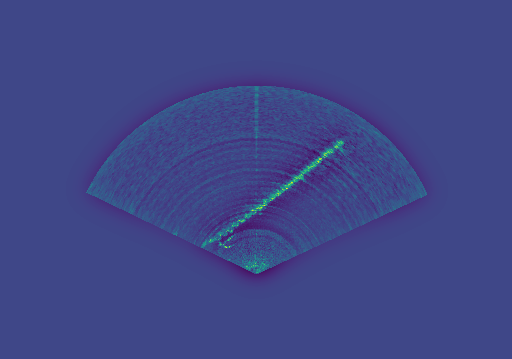
\includegraphics[width=\textwidth]{figures/bandpassing/0_10.png}
        \caption{\(\sigma_{low} = 0\) \(\sigma_{high} = 10\)}
    \end{subfigure}
    \hfill
    \begin{subfigure}[b]{.32\textwidth}
        \centering
        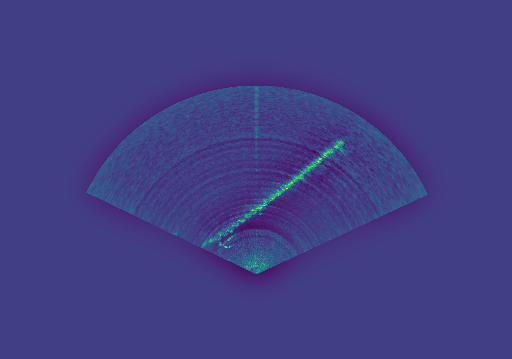
\includegraphics[width=\textwidth]{figures/bandpassing/0_15.png}
        \caption{\(\sigma_{low} = 0\) \(\sigma_{high} = 15\)}
    \end{subfigure}
    \hfill
    \begin{subfigure}[b]{.32\textwidth}
        \centering
        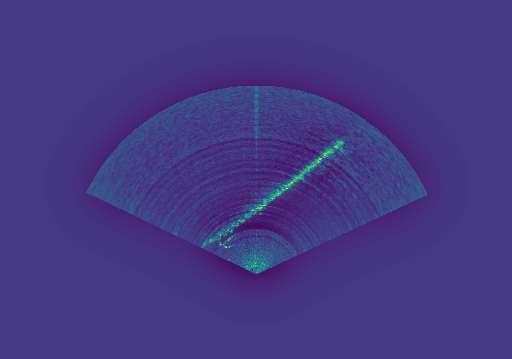
\includegraphics[width=\textwidth]{figures/bandpassing/0_20.png}
        \caption{\(\sigma_{low} = 0\) \(\sigma_{high} = 20\)}
    \end{subfigure}
    \hfill
    \begin{subfigure}[b]{.32\textwidth}
        \centering
        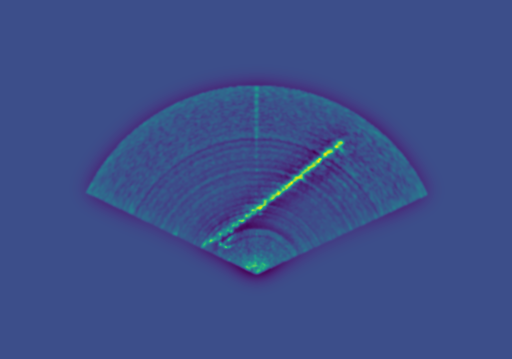
\includegraphics[width=\textwidth]{figures/bandpassing/1_10.png}
        \caption{\(\sigma_{low} = 1\) \(\sigma_{high} = 10\)}
    \end{subfigure}
    \hfill
    \begin{subfigure}[b]{.32\textwidth}
        \centering
        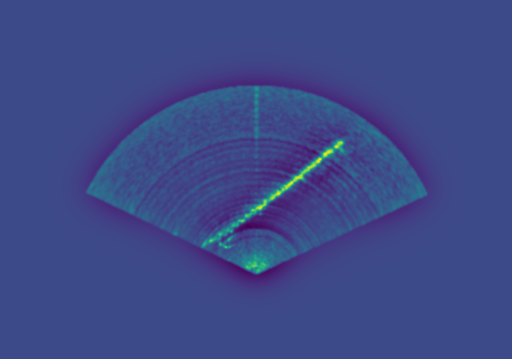
\includegraphics[width=\textwidth]{figures/bandpassing/1_15.png}
        \caption{\(\sigma_{low} = 1\) \(\sigma_{high} = 15\)}
    \end{subfigure}
    \hfill
    \begin{subfigure}[b]{.32\textwidth}
        \centering
        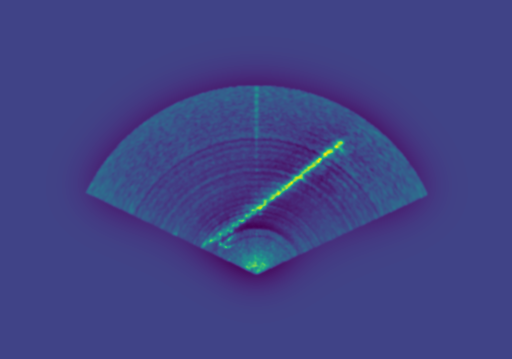
\includegraphics[width=\textwidth]{figures/bandpassing/1_20.png}
        \caption{\(\sigma_{low} = 1\) \(\sigma_{high} = 20\)}
    \end{subfigure}
    \hfill
    \begin{subfigure}[b]{.32\textwidth}
        \centering
        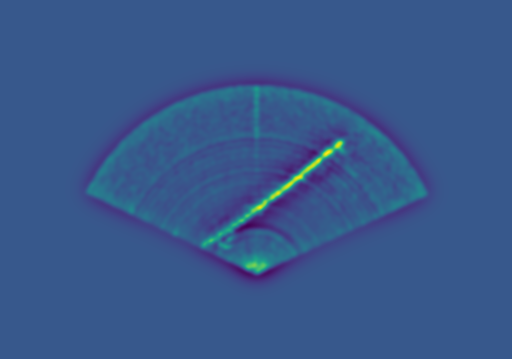
\includegraphics[width=\textwidth]{figures/bandpassing/2_10.png}
        \caption{\(\sigma_{low} = 2\) \(\sigma_{high} = 10\)}
    \end{subfigure}
    \hfill
    \begin{subfigure}[b]{.32\textwidth}
        \centering
        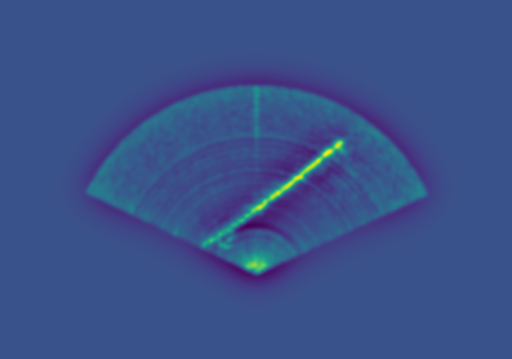
\includegraphics[width=\textwidth]{figures/bandpassing/2_15.png}
        \caption{\(\sigma_{low} = 2\) \(\sigma_{high} = 15\)}
    \end{subfigure}
    \hfill
    \begin{subfigure}[b]{.32\textwidth}
        \centering
        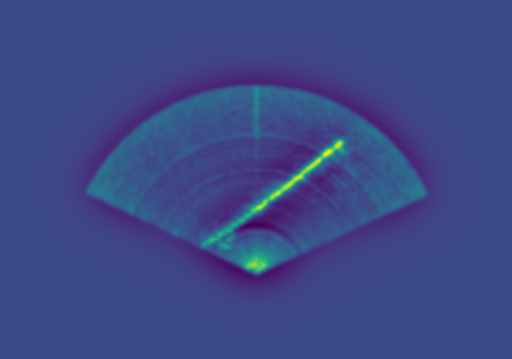
\includegraphics[width=\textwidth]{figures/bandpassing/2_20.png}
        \caption{\(\sigma_{low} = 2\) \(\sigma_{high} = 20\)}
    \end{subfigure}
    \hfill
    \begin{subfigure}[b]{.32\textwidth}
        \centering
        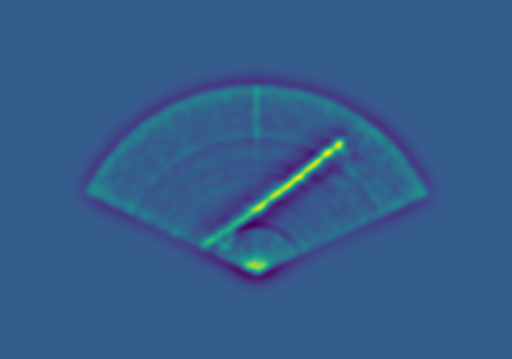
\includegraphics[width=\textwidth]{figures/bandpassing/3_10.png}
        \caption{\(\sigma_{low} = 3\) \(\sigma_{high} = 10\)}
    \end{subfigure}
    \hfill
    \begin{subfigure}[b]{.32\textwidth}
        \centering
        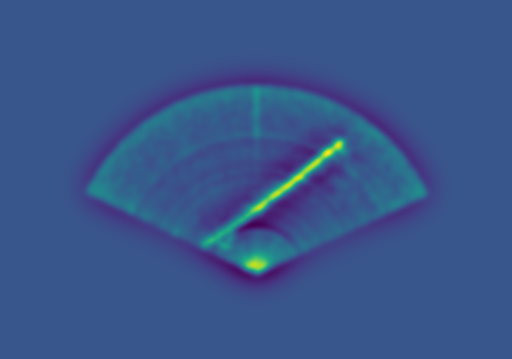
\includegraphics[width=\textwidth]{figures/bandpassing/3_15.png}
        \caption{\(\sigma_{low} = 3\) \(\sigma_{high} = 15\)}
    \end{subfigure}
    \hfill
    \begin{subfigure}[b]{.32\textwidth}
        \centering
        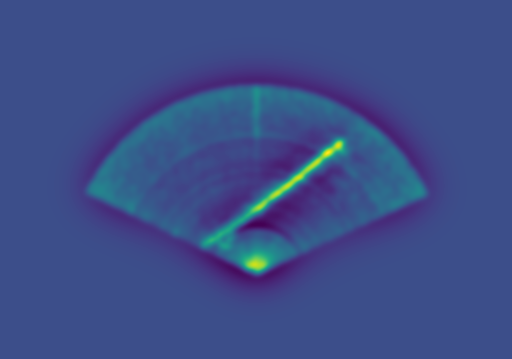
\includegraphics[width=\textwidth]{figures/bandpassing/3_20.png}
        \caption{\(\sigma_{low} = 3\) \(\sigma_{high} = 20\)}
    \end{subfigure}
    \caption{Choosing \(\sigma_{low}\) and \(\sigma_{high}\) values for band-passing}
\end{figure}

Combination \(\sigma_{low} = 2\) \(\sigma_{high} = 20\) is chosen as it accentuates contrast between empty background and features without losing too much detail in the blurring. It's very hard to justify why these parameters would best quantitatively. The metric to go to in this case would be \acrfull{snr}. However this is impossible to calculate without having a reference "true" signal. These parameters can be changed easily from the \acrshort{cli} if desired. In code this filter is implemented through the \texttt{skimage.filters.difference\_of\_gaussians} package:

\begin{lstlisting}[
    caption={Bandpassing code.},
    label=lst:pipeline-bandpassing,
    language=Python]
difference_of_gaussians(img, low_sigma, high_sigma)
\end{lstlisting}

Once more, this is a perfect candidate for parallelization using \texttt{Ray}.

\subsection{Masking}

As mentioned before, when applying a discrete Fourier transform if the input isn't periodic this might result in "spectral leakage". This shows up as random frequencies that aren't really part of the input. To avoid this, some windowing of the image is required. As part of the inputs of the pipeline a mask is provided which might be transformed by some of the modules. For example the Fan Transformation Module will convert the rectangular input mask into the fan shape. By default the input mask to the pipeline is an array of ones with the same shape as a sonar frame. The masking module takes the input mask, reduces the size of the masking area while preserving the image size, and applies some gaussian filtering to it with the purpose of smoothing its edges:

\begin{figure}[H]
    \centering
    \begin{subfigure}[b]{.45\textwidth}
        \centering
        
\includegraphics[width=\textwidth]{figures/pipeline/Mask.png}
        \caption{Fan mask.}
    \end{subfigure}
    \hfill
    \begin{subfigure}[b]{.45\textwidth}
        \centering
        
\includegraphics[width=\textwidth]{figures/pipeline/MaskBlurred.png}
        \caption{Smoothed \& resized mask.}
    \end{subfigure}
    \caption{Smoothing the mask.}
    \label{fig:mask-smoothing}
\end{figure}

A padding of \texttt{60px} on every side was chosen as after resizing back to the orignal image size, it makes the blurred border fit completely inside the original mask. In code this is implemented using \texttt{numpy}, \texttt{scipy.ndimage.gaussian\_filter} and \texttt{skimage.transform.resize}:

\begin{lstlisting}[
    caption={Smoothed mask code.},
    label=lst:pipeline-masking-smoothing,
    language=Python]
# Add black border
padding = 60
mask = np.pad(input_mask, padding, mode='constant', constant_values=0)
# Resize mask to orignal size
mask = resize(mask, input_mask.shape, anti_aliasing=True)
# Gaussian blur the mask
mask = gaussian_filter(mask, sigma=self.sigma)
\end{lstlisting}

Another optimization takes place here. Instead of recalculating this mask for every incoming frame, the mask is cached and reused in the future. The caching implementation is very simple so the restriction of all frames being the same size still applies. This mask is then applied to the input frames to reduce the visibility of the border of the sonar frame:

\begin{figure}[H]
    \centering
    \begin{subfigure}[b]{.45\textwidth}
        \centering
        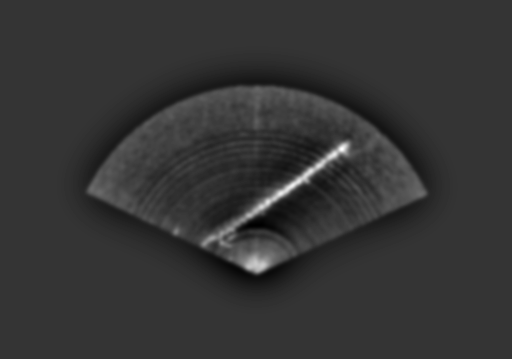
\includegraphics[width=\textwidth]{figures/pipeline/Bandpass.png}
        \caption{Unmasked frame.}
    \end{subfigure}
    \hfill
    \begin{subfigure}[b]{.45\textwidth}
        \centering
        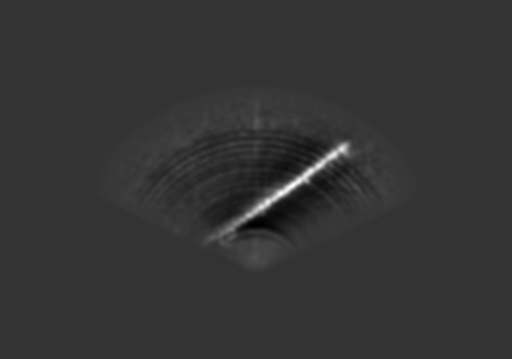
\includegraphics[width=\textwidth]{figures/pipeline/Masking.png}
        \caption{Masked frame.}
    \end{subfigure}
    \caption{Applying the mask.}
    \label{fig:mask-application}
\end{figure}

Using \texttt{numpy} this can be easily achieved through element-wise multiplication: \lstinline{image * mask}. Yet again, except for the calculation of the mask the first time the module runs, this is a perfect candidate for parallelization using \texttt{Ray}.

\section{Fan Transformation}
One of the main modules is definitely the Fan Transformation Module. The raw data from the sensor is structured in an array that represents ping intensity at a specific bearing and range. It is important to note that the beam bearings are not evenly spaced. The sensor provides a table that accompanies the ping information with the specific angle associated with each ping. All of this data is obtained through recording files stored on the \acrshort{rov}. These files contain the sonar data packed in a "Protocol Buffers" format specified by Blueye's Protocol Definitions \cite{Blueye:ProtocolDefinitions}. The following is an example "MultibeamPing" message:

\begin{lstlisting}[
    caption={Example MultibeamPing message.},
    label=lst:ping-protobuf]
ping {
  range: 30.758804321289062
  gain: 100.0
  frequency: 1196808.5106382978
  speed_of_sound_used: 1517.4982581645493
  frequency_mode: MULTIBEAM_FREQUENCY_MODE_LOW_FREQUENCY
  number_of_ranges: 378
  number_of_beams: 512
  step: 512
  bearings: -65.0
  bearings: -64.5199966430664
  ...
  bearings: 64.5199966430664
  bearings: 65.0
  ping_data: [1D array containing sonar image]
  device_id: GUEST_PORT_DEVICE_ID_BLUEPRINT_SUBSEA_OCULUS_M1200D
}
\end{lstlisting}

The \lstinline{ping_data} is produced as a continuous 1D array that must be reshaped in order to work with it as an image. Using the \lstinline{number_of_ranges} and \lstinline{number_of_beams} we can convert the 1D-array into a 2D one. Using the equations from \ref{sec:fan-tform} and the bearing table provided by the MultibeamPing record, the fan transformation can be implemented as a module in the pipelines. 

A huge optimization can be performed here. Given the restriction that all the frames should have the same range and number of beams, the mapping can be pre-computed for all images and cached for use on all the incoming frames. This saves cpu cycles on performing all the possible \((u, v) \rightarrow (\theta,r)\) calculations. The effect of this speedup will be evaluated in the following sections.

Range resolution depends on the sonar, in our case 2.5mm per pixel along the range axis \ref{tab:sonar_specs}. It allows us to convert simple pixel values into real world coordinates. In most cases, a simple division of \lstinline{range} over \lstinline{number_of_ranges} will give us this value. However, it is often the case that to speed up processing images are resized. If the image is scaled a simple calculation can compensate for this change. Given \(R\) as the resizing ratio for the image area, the resizing ratio for a dimension of the image will be given by \(\sqrt{R}\). The new range resolution can be calculated with the following equation:

\[rangeResolution = \frac{range}{numberOfRanges * \sqrt{R}}\]

This module is yet another example of a candidate for parallelization using \texttt{Ray}.

\section{Registration Modules}



\subsection{\acrfull{fft}}

\begin{figure}[H]
    \centering
    \begin{subfigure}[b]{.45\textwidth}
        \centering
        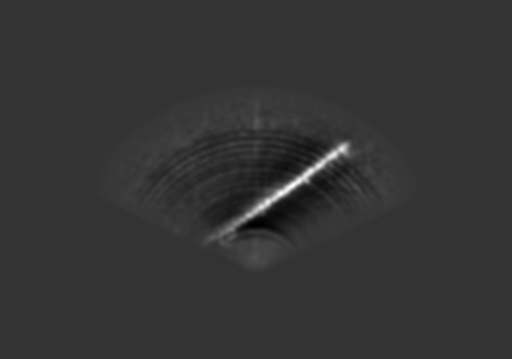
\includegraphics[width=\textwidth]{figures/pipeline/Masking.png}
        \caption{Masked frame.}
    \end{subfigure}
    \hfill
    \begin{subfigure}[b]{.45\textwidth}
        \centering
        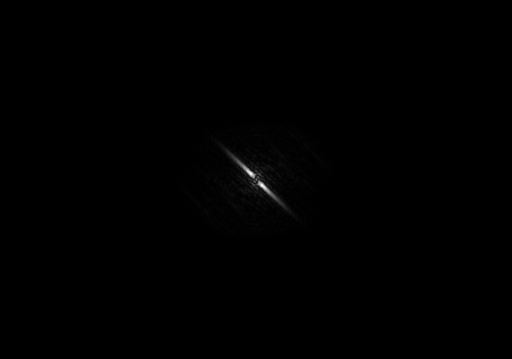
\includegraphics[width=\textwidth]{figures/pipeline/FFT.png}
        \caption{FFT.}
    \end{subfigure}
    \caption{Fourier transform.}
    \label{fig:fft}
\end{figure}

A simple module that applies the \acrshort{fft} to incoming inputs. The \acrshort{fft} is an algorithm that implements the Discrete Fourier Transform efficiently. The result of the transform is a signal in the complex domain (composed of Real and Imaginary parts). Decomposition into magnitude and phase makes it easier to visualize, and as mentioned previously in \autoref{sec:fm-registration} we're only interested in the magnitude for rotation estimation using \citeauthor{Reddy1996}'s Fourier-Mellin Pipeline. Using \texttt{numpy} we can get the magnitude of the \acrshort{fft} and center the zero-frequency component with:

\begin{lstlisting}[
    caption={FFT.},
    label=lst:pipeline-fft,
    language=Python]
np.abs(np.fft.fftshift(np.fft.fft2(image)))
\end{lstlisting}

\subsection{Log-Polar Transform}

\begin{figure}[H]
    \centering
    \begin{subfigure}[b]{.45\textwidth}
        \centering
        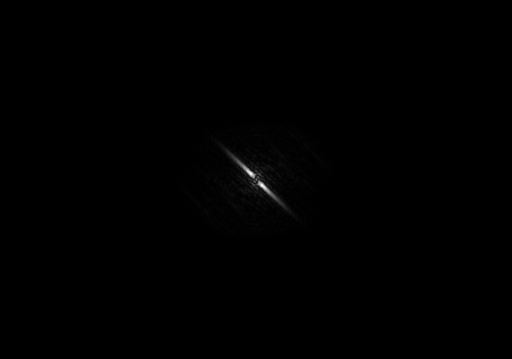
\includegraphics[width=\textwidth]{figures/pipeline/FFT.png}
        \caption{FFT.}
    \end{subfigure}
    \hfill
    \begin{subfigure}[b]{.45\textwidth}
        \centering
        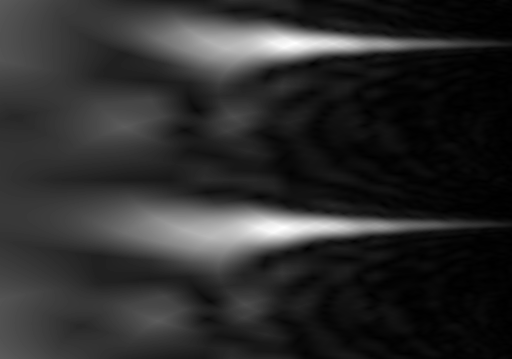
\includegraphics[width=\textwidth]{figures/pipeline/LogPolar.png}
        \caption{Log-Polar Transform of FFT.}
        \label{sfig:log-polar}
    \end{subfigure}
    \caption{Log-Polar Transform.}
    \label{fig:log_polar}
\end{figure}

The log polar transform is module used only in the Fourier-Mellin approach. Together with the \acrshort{fft} and phase correlation it can be to estimate the rotation of the image. In the project this is implemented using \texttt{skimage.transform.warp\_polar}:

\begin{lstlisting}[
    caption={Log Polar Transform.},
    label=lst:pipeline-log-polar,
    language=Python]
warp_polar(data, radius=radius, scaling='log', order=order, output_shape=shape)
\end{lstlisting}

The radius \lstinline{radius} must be chosen as a fraction of the height of the input image. By choosing 1/8th of the height, most of the areas without data (black) are removed from the output image. 


\subsection{Phase Correlation}

At the phase correlation step the only thing that is calculated is the translation between the source images. What this translation means actually depends on the input images and the parameter that's being estimated.

\begin{figure}[H]
    \centering
    \begin{subfigure}[b]{.45\textwidth}
        \centering
        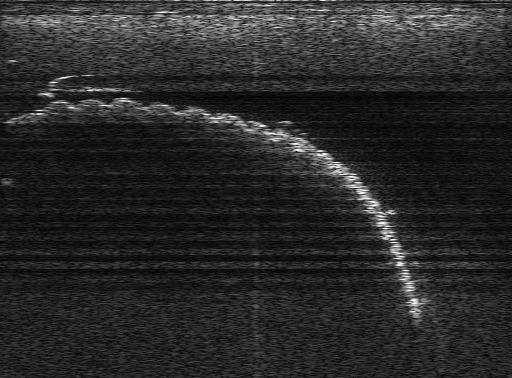
\includegraphics[width=\textwidth]{figures/pipeline/Original.png}
        \caption{Raw frame.}
    \end{subfigure}
    \hfill
    \begin{subfigure}[b]{.45\textwidth}
        \centering
        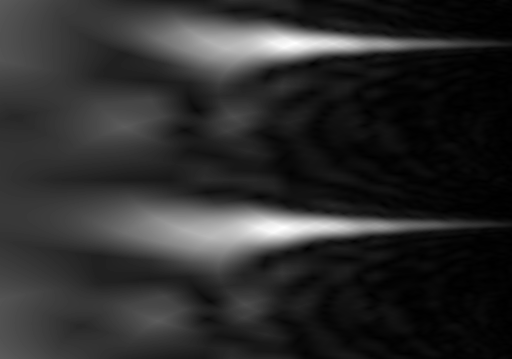
\includegraphics[width=\textwidth]{figures/pipeline/LogPolar.png}
        \caption{Log-Polar Transform of FFT.}
    \end{subfigure}
    \caption{Rotation estimation.}
    \label{fig:rotation-estimation}
\end{figure}

If Phase Correlations is being used to estimate rotations, the axis to choose depends on the input. As can be seen in \autoref{fig:rotation-estimation}, and remembering what has been mentioned in \autoref{sec:fan-tform}, for a raw sonar frame the \(\theta\) axis is the horizontal one. Meanwhile, the Log-Polar Transform is represented by \(\log{\rho}\) on the horizontal axis and \(\theta\) on the vertical one. 

In both cases, the output of Phase Correlation describes the translation in the \(\theta\) axis as distance in pixels. This must be scaled to actual degrees.

For the Log-Polar Transform the whole axis represent 360º, while for the raw sonar frame it only represents the \acrfull{fov}. This value can be retrieved from the \autoref{tab:sonar_specs} or from the bearings table by subtracting the maximum an minimum value for the bearings. 

Using \texttt{skimage.registration.phase\_cross\_correlation} and \texttt{numpy} the code can be implemented in the following manner:

\begin{lstlisting}[
    caption={Phase Correlation.},
    label=lst:pipeline-phase-correlation,
    language=Python]
shifts, e, _ = phase_cross_correlation(a, b, upsample_factor=self.upsample_factor)
\end{lstlisting}

This function returns not only the translational shift but also an error measurement which is an indication of the confidence of the measurement.

The angle estimation can be done like so (note how the chosen axes are different): 
\begin{lstlisting}[
    caption={Phase Correlation.},
    label=lst:pipeline-phase-correlation-rotation,
    language=Python]
if self.log_polar:
    angle = shifts[0] * 360 / a.shape[0]
else:
    fov = 130
    angle = shifts[1] * fov / a.shape[1]
\end{lstlisting}

At this point a \texttt{SimilarityTransform} must be created to represent this translation. This rotation should be applied around the center of the image. To do this three steps must be followed:
\begin{enumerate}
    \item Apply a translation from the image center to the origin (\(T_1\)).
    \item Apply the rotation (\(R\)).
    \item Apply a translation back to the original location (\(T_2\)).
\end{enumerate}

This can be executed in code using \texttt{skimage.transform.SimilarityTransform}:
\begin{lstlisting}[
    caption={Phase Correlation.},
    label=lst:pipeline-phase-correlation-tform,
    language=Python]
tform = SimilarityTransform(translation=-center)
tform += SimilarityTransform(rotation=np.deg2rad(angle))
tform += SimilarityTransform(translation=center)
\end{lstlisting}

For the estimation of translations the code is much simpler since the output of the Phase Correlation step is already usable data. To add this translation to the \lstinline{tform} defined in the previous step the following code can be used:
\begin{lstlisting}[
    caption={Phase Correlation.},
    label=lst:pipeline-phase-correlation-tform-2,
    language=Python]
tform += SimilarityTransform(translation=[shifts[1], shifts[0]])
\end{lstlisting}

The resulting \lstinline{tform} is the full transform that is needed to register the input frames. 

\subsection{Warping}
\label{sec:warping}

The warping step uses \texttt{skimage.transform.warp} to apply an input transform to the image. It is applied only to the incoming frame and is achieved with the following code:

\begin{lstlisting}[
    caption={Warping.},
    label=lst:pipeline-warp,
    language=Python]
b = warp(b, tform.inverse, output_shape=b.shape)
\end{lstlisting}

Since the transform \lstinline{tform} represents what the first frame (a) needs to do to batch the most recent one (b), it must be inverted to bring everything back into the reference frame of (a).


\section{Mosaicing}

The process of mosaicing the images is straightforward. Having calculated the position of an incoming frame, warp this frame to place it with the previous ones on a combined map. However, two main questions arise:

\begin{itemize}
    \item How to handle images going beyond the "border" of the currently known world? Naive approaches to mosaicing might start with a fixed sized canvas to combine the images. If the sonar were to move beyond this limit, it would be imposible to render this data.
    \item How to merge overlapping data? It will most likely be the case that many images will have significant overlap. Just taking the latest one would discard a lot of usable data, and naive averaging of the whole image might have unintended side effects.
\end{itemize}

\subsection{Handling borders}
The simplest solution to solve the question of borders is to make the canvas grow with the images as they are placed. The simplest way to do this is to calculate the position of the corners of the image given its transform and if it goes beyond the image, determine how much padding is needed. It is important to remember that in this case the \(y\) axis is inverted (positive is downwards).

\begin{figure}[H]
    \centering
    \begin{subfigure}[b]{.45\textwidth}
        \centering
        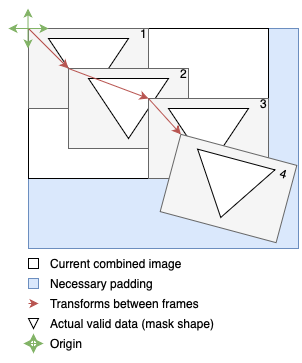
\includegraphics[width=\textwidth]{figures/mosaicing/Mosaicing.png}
        \caption{Padding in positive direction.}
        \label{sfig:mosaic-positive}
    \end{subfigure}
    \hfill
    \begin{subfigure}[b]{.45\textwidth}
        \centering
        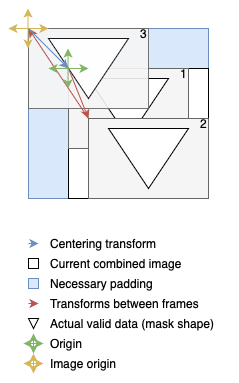
\includegraphics[width=\textwidth]{figures/mosaicing/Centering.png}
        \caption{Padding in negative direction.}
        \label{sfig:mosaic-negative}
    \end{subfigure}
    \caption{Mosaicing depending on the direction of the padding.}
    \label{fig:mosaicing}
\end{figure}

The following cases are possible:

\begin{itemize}
    \item All of the corners fit inside the current combined image. No padding required.
    \item A corner has a positive \(x\) or \(y\) coordinate that goes beyond the size of the current combined image as in \autoref{sfig:mosaic-positive}. The combined image must be padded along the respective axis, while preserving the current origin. The padding amount is determined by the difference of either the current width/height and the coordinate. The centering transform remains unaffected.
    \item A corner has a negative coordinate like in \autoref{sfig:mosaic-negative}. The combined image must be padded along the corresponding axis, but this won't preserve the origin. Since future transforms between frames will still come in the Origin reference frame (green), the centering transform must be updated to correctly position the Origin with respect to the Image Origin (yellow).
\end{itemize}

To not evaluate this over every corner, it is better to find a bounding box around the corners by finding the \(x\) and \(y\) coordinate with the minimum and maximum values respectively. The previous rules apply now over these four values. In Python we can find these corners using \texttt{skimage.transform.SimilarityTransform} and \texttt{numpy}, and use them to perform padding and centering of the image:

\begin{lstlisting}[
    caption={Detecting incoming frame corner position.},
    label=lst:pipeline-mosaicing-corners,
    language=Python]

# Calculate corners position
source_corners = np.array([[0, 0], 
                           [0, img.shape[0]], 
                           [img.shape[1], img.shape[0]], 
                           [img.shape[1], 0]])
corners = (centering_tform + total_tform)(source_corners)

# Find bounding box
max_x = np.max(corners[:, 0])
min_x = np.min(corners[:, 0])
max_y = np.max(corners[:, 1])
min_y = np.min(corners[:, 1])

# Determine padding
left = int(np.abs(min_x)) if min_x < 0 else 0
right = int(max_x - combined.shape[1] - 1) if max_x >= combined.shape[1] else 0
top = int(np.abs(min_y)) if min_y < 0 else 0
bottom = int(max_y - combined.shape[0] - 1) if max_y >= combined.shape[0] else 0

# Update centering transform
centering_tform = SimilarityTransform(translation=(left, top)) + centering_tform

# Pad combined image to fit new corners
combined = np.pad(combined, 
                  ((top, bottom), (left, right)), 
                  mode='constant', 
                  constant_values=0)
\end{lstlisting}

In the \autoref{lst:pipeline-mosaicing-corners} the \lstinline{img} refers to the incoming frame, \lstinline{combined} to the mosaic, \lstinline{centering_tform} to the transform between the Image Origin (yellow) and the Origin (green), and \lstinline{total_tform} represents the concatenated transforms between frames. 

Now that the combined image is of the right size the incoming frame can be warped similarly to \autoref{sec:warping}. To combine them we will refer to the next section.

\subsection{Merging data}

As mentioned in \autoref{sec:mosaicing}, averaging the incoming frames yields good results in terms of SNR improvements. However, averaging the incoming frames is not as straightforward as simply averaging the warped frame from the last section with the combined image. The only values that can actually be averaged are those within the area defined by the mask. Since everything outside the mask is black, if this data were to be included it would tend to attenuate the brightness of the combined image, and possibly lose data. This can be achieved using \texttt{numpy} through a three step process:
\begin{enumerate}
    \item Warping the incoming frame and resizing it to the size of the combined frame.
    \item Convert all of the values outside the mask to \lstinline{np.nan} using array masking.
    \item Use \texttt{numpy}'s nan-operators like \lstinline{np.nansum}, \lstinline{np.isnan}, etc. to combine the images.
\end{enumerate}

There is another important consideration to keep in mind. In a streaming setup, where only the combined image and the incoming frame are available, these two can't simply be averaged. This would give too much importance to the incoming image while decreasing the contribution of older ones. For example, by the time the 5th frame comes in, the first one will only contribute to 6.25\% of the data:
\begin{itemize}
    \item 1: 100\%
    \item 2: 50\%, 1: 50\%
    \item 3: 50\%, 2: 25\%, 1: 25\%
    \item 4: 50\%, 3: 25\%, 2: 12.5\%, 1: 12.5\%
    \item 5: 50\%, 4: 25\%, 3: 12.5\%, 2: 6.25\%, 1: 6.25\%
\end{itemize}

A weighted average is required to make all the images equally important. Although at the point of combining the images it is hard to know how many are actually overlapping, an improvement over the naive approach is to use the total count of merged images to calculate the weights. Given \(N\) frames in the most recent combined image, the weights for the new combined map and incoming frame are:

\[w_{combined} = \frac{N}{N + 1}\]
\[w_{incoming} = \frac{1}{N + 1}\]
\[I_{combined}' = I_{incoming} * w_{incoming} + I_{combined} * w_{combined} \]

As mentioned before, this should only be applied to the area of the image that falls inside the mask. The values outside this area can also be forced to take their previous value by using the mask. In code we can do this like so:

\begin{lstlisting}[
    caption={Averaging images in mosaic.},
    label=lst:pipeline-mosaicing-averaging,
    language=Python]
# Resize mask 
mask = warp(mask, SimilarityTransform(), output_shape=img.shape)
# Make values outside of mask np.nan
img[mask < 1] = np.nan
# Warp image and make all values outside of image np.nan
# (The warp method requires using the inverse of the transform)
img = warp(img, 
           (centering_tform + total_tform).inverse, 
           output_shape=combined.shape, 
           mode='constant', 
           cval=np.nan)

# Weighted previous combined image
previous_combined = combined * (combined_count / combined_count + 1))
# Force values outside mask to remain the same
previous_combined[np.isnan(img)] = combined[np.isnan(img)]
# Weighted incoming frame
next_frame = img / (self.find_root().combined_count + 1)
# Resulting combined image
combined = np.nansum(np.dstack((previous_combined, next_frame)), 2)
\end{lstlisting}

After this is done, the count of combined frames should be updated.